
\begin{figure*}[h]
	\centering
	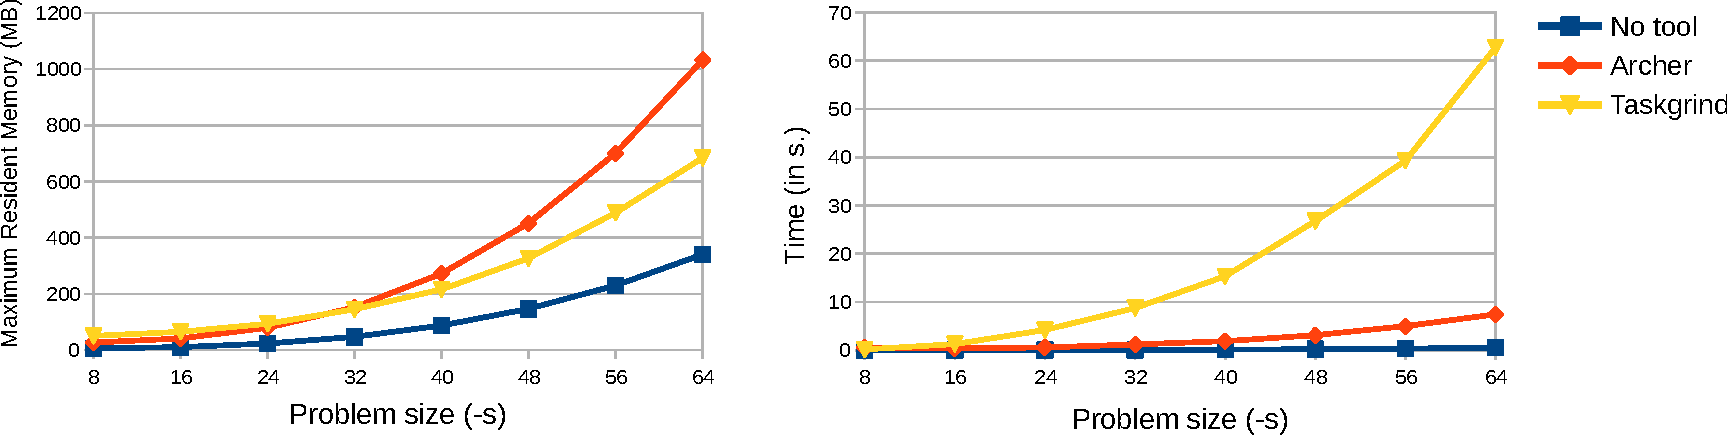
\includegraphics[width=\linewidth]{../figures/lulesh.pdf}
	\caption{Execution Time and Memory overheads on LULESH with parameters `-s \$s -tel 4 -tnl 4 -p -i 4`}
	\label{fig:lulesh}
\end{figure*}


% Lulesh parameters were :  -s 16 -tel 4 -tnl 4 -p -i 4
\begin{table*}[]

	\centering
	\small
	\begin{tabular}{cc|ccc|ccc|cc}
		\multicolumn{1}{l}{}     & \multicolumn{1}{l|}{}              & \multicolumn{3}{c|}{Execution time (s.)}                                                   & \multicolumn{3}{c|}{Memory usage (MB.)}                                                    & \multicolumn{2}{c}{N° of reports} \\ \hline
		\multicolumn{1}{l}{Racy} & \multicolumn{1}{l|}{N° of threads} & \multicolumn{1}{l}{No tools} & \multicolumn{1}{l}{Archer} & \multicolumn{1}{l|}{Taskgrind} & \multicolumn{1}{l}{No tools} & \multicolumn{1}{l}{Archer} & \multicolumn{1}{l|}{Taskgrind} & Archer           & Taskgrind      \\
		\multirow{2}{*}{no}      & 1                                  & 0.01                         & 0.12                       & 1.23                           & 10                           & 41                         & 64                             & 0                & 0              \\
		& 4                                  & 0.01                         & 0.43                       & \emph{deadlock}                       & 15                           & 83                         & \emph{deadlock}                       & 149 to 273       & \emph{deadlock}       \\
		\multirow{2}{*}{yes}     & 1                                  & 0.01                         & 0.12                       & 1.23                           & 10                           & 41                         & 64                             & 0                & 458            \\
		& 4                                  & 0.01                         & 0.46                       & \emph{deadlock}                       & 15                           & 84                         & \emph{deadlock}                       & 140 to 221       & \emph{deadlock}
	\end{tabular}
	\caption{Execution time, memory usage overheads and number of reports for Archer and Taskgrind, on a dependent task-based OpenMP implementation of LULESH with -s 16 -tel 4 -tnl 4 -p -i 4}
	\label{tbl:results-lulesh}
\end{table*}

%%%%%%%%%%%%%%%%%%%%%%%%%%%%%%%%%%%%%%%%%%%%%%%%%%%%%%%%%%%%%%%%%%%%%%%%%%%%%%
\section{Evaluation} \label{sec:eval}
%%%%%%%%%%%%%%%%%%%%%%%%%%%%%%%%%%%%%%%%%%%%%%%%%%%%%%%%%%%%%%%%%%%%%%%%%%%%%%

The original motivations of Taskgrind were to have no false negative reports (as compared to Archer and TaskSanitizer) - while improving error reports (as compared to ROMP).
This section evaluates Taskgrind determinacy race analysis, its overhead over execution time, and memory use, and illustrates its error reporting capabilities\footnote{Software versions and source code are referenced in the Appendix of this document.}.
Every program was compiled using LLVM and disabling optimizations (option \code{-O0}).

% - . - . - . - . - . - . - . - . - . - . - . - . - . - . - . - . - . - . - .%
\subsection{Microbenchmarks}
% - . - . - . - . - . - . - . - . - . - . - . - . - . - . - . - . - . - . - .%
We evaluate Taskgrind determinacy race detection analysis on a subset of the DataRaceBenchmarks~\cite{drb} focusing on task-related constructs.
We extended it with seven Taskgrind-specific microbenchmarks (TMB) treating heavyweight DBI pitfalls discussed in \sect{sec:pitfalls}.
We run TMBs with 1 and 4 threads to:
\begin{itemize}
	\item	force memory recycling, thread-local accesses, and segment-local accesses of independent segments,
	\item 	ensures the tool captures the code semantic and not implementation specific behavior.
	For instance, LLVM implementation makes every task \emph{included} when executing on a single-thread~\footnote{\url{https://github.com/llvm/llvm-project/issues/89398}}.
\end{itemize}
Results are depicted on \tbl{tbl:results-race-detection} and confront state-of-the-art analysis tools: TaskSanitizer~\cite{Matar18}, Archer~\cite{archer} and ROMP~\cite{ROMP}.
The first column is the benchmark name, the second is whether a data race is present, and the other columns depict reports obtained by the specified tools.
Letter $(T, F, P, N)$ respectively stands for ($true$, $false$, $positive$, $negative$).
\emph{ncs} on TaskSanitizer stands for "no compiler support" and indicates that the test does not compile with Clang 8.x.
\emph{segv} on ROMP indicates that the instrumented execution was incomplete due to a run-time error.

As Taskgrind's main objective is to avoid false negative reports, we have highlighted them.
Amongst all the tools, it reports the least false-negative with only a single one on \emph{DRB129-mergeable-taskwait-orig}.
It evaluates the support for OpenMP \code{mergeable} clause, which semantic is not supported by Taskgrind, nor by TaskSanitizer, Archer, or ROMP.
Single-thread execution of TMB reports 100\% accuracy, while other tools do not.
The multi-threaded execution of TMP reports a few false positives that require further investigation: Taskgrind detects conflicting sibling tasks on a memory location in their parent segment stack frame.

%129 - mergeable - the llvm implementation we had was not merging data environment, so no determinacy race detected: two distincts data environment are being accessed. - if we wanted to detect this, we should add the data environement and mergeable clause semantic to taskgrind.
%TODO : can OMPT tell us the mapping between two data environement to detect such issue ?
%
%131, 134, 165 - if(0) undefered clause, not supported when num-threads == 0 by LLVM

% - . - . - . - . - . - . - . - . - . - . - . - . - . - . - . - . - . - . - .%
\subsection{LULESH}
% - . - . - . - . - . - . - . - . - . - . - . - . - . - . - . - . - . - . - .%
\tbl{tbl:results-lulesh} and \fig{fig:lulesh} reports data race detection and overheads on execution time and memory usage on the LULESH proxy application on 12th Gen Intel(R) Core(TM) i5-12450H.
The execution time reported for Taskgrind only includes the recording phase and not the determinacy race analysis.

On the table, we report two versions of LULESH: a correct one (with \emph{no} in the "racy" column) and an incorrect one (with \emph{yes} in the "racy" column) by removing a task dependence to introduce data races intentionally.
We also run it on 1 and 4 threads for the same reason as the previous experiment.
On the single-threaded run, we observe a slowdown against non-instrumented versions of $10x$ for Archer and $100x$ for Taskgrind and a memory overhead of $4x$ for Archer and $6x$ for Taskgrind.
The reasons for Taskgrind deadlocks running with multiple threads remain to be investigated.
Regarding data race, Archer never reports errors when running in a single-thread, most likely because it only sees undeferred tasks through OMPT due to LLVM serialization.
On the other hand, we annotated the code to notify Taskgrind that the task is semantically deferrable, which leads to no false negatives on the racy version with 458 races detected.

On the figure, the x-axis varies the problem size \code{-s} - with the application having a $O(s^3)$ time and memory complexity.
The reference and Archer execute with four threads, and Taskgrind with a single thread.

We also evaluated using ROMP but omitted results from the figure, as the instrumented program crashed early during the first iteration of LULESH.
Still, measurements showed that memory use and execution time follow a similar shape with \code{s}, but with much larger overheads: for \code{-s=64}, before the application crashes, the execution time and memory use were respectively $79 s$ and $75GB$.


% - . - . - . - . - . - . - . - . - . - . - . - . - . - . - . - . - . - . - .%
\subsection{Error Reporting}
% - . - . - . - . - . - . - . - . - . - . - . - . - . - . - . - . - . - . - .%

\listing{lst:error-report} is a minimal erroneous OpenMP program, where the tasks line 8 and 11 may both concurrently access $x$.
\listing{lst:error-report-romp} and \listing{lst:error-report-taskgrind} respectively transcribe errors reported by ROMP and Taskgrind, compiling with debug symbols (option \code{-g}).
As you can see, Taskgrind provides debug information thanks to the Valgrind framework, while ROMP does not by default even though its DBI framework (Dyninst) can be patched to enable similar report.

%\begin{minipage}{\linewidth}
\begin{lstlisting}[style=CStyle, captionpos=b, caption={task.c - an errorneous OpenMP Program}, label={lst:error-report}]
int main(void)
{
	int * x = (int *) malloc(2 * sizeof(int));
	<@\textcolor{mBlue}{\# pragma omp parallel}@>
	{
		<@\textcolor{mBlue}{\# pragma omp single}@>
		{
			<@\textcolor{mBlue}{\# pragma omp task}@>
				x[0] = 42;
			
			<@\textcolor{mBlue}{\# pragma omp task}@>
				x[0] = 43;
		}
	}
	return 0;
}
\end{lstlisting}
%\end{minipage}

%\begin{minipage}{\linewidth}
\begin{lstlisting}[style=text, captionpos=b, caption={An error report from ROMP}, label={lst:error-report-romp}]
	[...]
	data race found:
\end{lstlisting}
%\end{minipage}

%\begin{minipage}{\linewidth}
\begin{lstlisting}[style=text, captionpos=b, caption={An error report from Taskgrind}, label={lst:error-report-taskgrind}]
	Segments task.1.c:8 and task.1.c:11 were declared independent while accessing the same memory address
	4 bytes from 0xC3EA040 allocated in block 0xC3EA040 of size 8
	from task.1.c:3
	[...]
\end{lstlisting}
%\end{minipage}



